\scanpage{103}
\mspage{102}

When $k$ is of characteristic zero, one always has a natural fibre functor: the \uline{Hodge functor,} which to the motivic cohomology of a (smooth projective) variety $X$ associates the bigraded vector space $\handwritten{\coprod}H^q(X,\handwritten{\underline{\Omega}}^p_{X/k})$ Thus for the corresponding motivic Galois group $G$, one finds a natural homomorphism\quad\handwritten{\tikz[baseline=0pt,x=1em,y=1em]{\draw (0,0)--(.12,.12);}}
\[
\underline{G}_m^2\handwritten{\longrightarrow}G,
\]
i.e. two homomorphisms commuting with one another\hspace{1em}\handwritten{\tikz[baseline=0pt,x=1em,y=1em]{\draw (.06,-.15)--(.1,-.32);\fill (0,-.4) circle (.045);}}
\[
i_1,i_2:\underline{G}_m\handwritten{\longrightarrow}G.
\]
The fact that the total grading in Hodge cohomology corresponds to the weight of motives is expressed by the relation
\[
i(\handwritten{\lambda})=i_1(\handwritten{\lambda})\,i_2(\handwritten{\lambda});
\]
one will bear in mind that $i_1$ and $i_2$ are not central (for the bigrading in Hodge cohomology does not correspond to a bigrading of a motive !)

2) Still taking $\underline{C}$ to be the c\rlap{t}a\rlap{a}t\rlap{g}egory of motives over $k$, w\unsure{\rlap{n}i|\rlap{m}i|i}th $k$ of characteristic zero, one has another canonical fibre functor, the \uline{De Rham functor}\rlap{\handwritten{\tikz[baseline=0pt,x=1em,y=1em]{\draw (0,-.7)--(.3,-.55);}}} which associates to the motivic cohomology of a variety $X$ the vector space $H^*(X,\handwritten{\Omega}^*_{X/k})$ (hypercohomology space). This vector space is no longer bigraded\rlap{\handwritten{\tikz[baseline=0pt,x=1em,y=1em]{\draw (0,-.65)--(.2,-.5);}}}\handwritten{\unsure{é,|en,|ée,}} but only graded and filtered,\rlap{x}\handwritten{(}the filtration being that associated with the hypercohomology spectral sequence, beginning with Hodge cohomology\rlap{x}\handwritten{)}. One knows moreover that this spectral sequence degenerates (Hodge theory), hence $\operatorname{Gr}(H_{\mathrm{DR}}(V))\handwritten{\simeq}H_{\mathrm{Hdg}}(V)$ (isomorphism functorial in the motive $V$\inserted{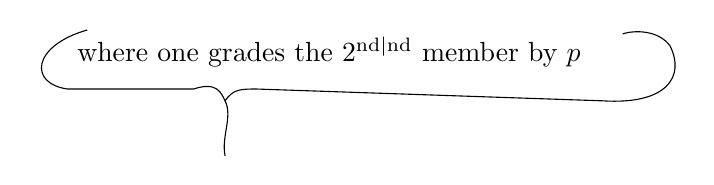
\begin{tikzpicture}[baseline=-.3ex,x=1cm,y=1cm]
\node[anchor=base west] at (0,.3) {\handwritten{where one grades the $2^{\unsure{\mathrm{nd}|\mathrm{nd}}}$ member \uline{by $p$}}};
\draw (.25,.7) .. controls (-.45,.5) and (-.5,.02) .. (0,-.05) -- (1.6,-.05) .. controls (1.9,.05) and (1.95,-.1) .. (2,-.2) .. controls (2.1,-.05) and (2.2,-.05) .. (2.4,-.05) -- (6.8,-.2) .. controls (7.6,-.25) and (7.85,.1) .. (7.65,.5) .. controls (7.5,.7) and (7.2,.7) .. (7.05,.65);
\draw (2,-.2) .. controls (2.1,-.4) and (1.95,-.65) .. (2,-.9);
\end{tikzpicture}}). One may set out to analyse to what additional structure, on the motivic Galois group associated with the fiber functor $H_{\mathrm{DR}}$, the canonical filtration of this functor corresponds.


In general, given a tensor category $C$ over $k$ \handwritten{\tikz[baseline=0pt,x=1em,y=1em]{\draw (0,.8)--(.15,1.02);}}equipped with a fibre functor $F$, one may set out to determine the filtra-
